% !TEX root = Theo_III.tex

\chapter{Elektrostatik}

Die Elektrostatik behandelt elektrische Felder ruhender oder langsam bewegter elektrischer Ladungen. In den folgenden Kapiteln werden die Grundgesetze der Elektrostatik aus dem Coulomb-Gesetz abgeleitet.

\section{Bemerkungen zur elektrischen Ladung}

Es gibt zwei Arten von Ladungen: positive und negative Ladung. Die Ladung ist eine diskrete Größe und nimmt stets ein ganzzahliges Vielfaches der sogenannten Elementarladung $e_{0}$ an:
\begin{equation*}
	e_{0}=\SI{1.602176624e-19}{\coulomb}
\end{equation*}
Diese wurde zuerst bei dem Millikan-Versuch bestimmt. So trägt zum Beispiel das Proton die Ladung $+e_{0}$ und das Elektron die Ladung $-e_{0}$. Quarks haben zwar Bruchteile der Elementarladung, treten aber nie frei, sondern nur in Kombinationen auf, die ein Vielfaches der Elementarladung bilden.

Es gilt strenge Ladungserhaltung:
\begin{formal}
	In einem abgeschlossenen System bleibt die Summe aller Ladungen konstant.
\end{formal}
Eine Ladung auf einem infinitesimalen Raum wird als Punktladung bezeichnet. In der Elektrostatik und der Elektrodynamik wird häufig mit der Ladungsdichte $\rho $ gerechnet. Für eine einzige Punktladung $q$ (zum Beispiel ein Proton oder Elektron) am Ort $\vec {r}_{0}$ gilt für die Ladungsdichteverteilung
\begin{equation*}
	\rho \left(\vec {r}\right)=q\delta \left(\vec {r}-\vec {r}_{0}\right).
\end{equation*}
Daraus lässt sich die Ladungsdichte für viele Punktladungen $q_{i}$ an Orten $\vec {r}_{i}$ verallgemeinern:
\begin{equation*}
	\rho \left(\vec {r}\right)=\sum _{i}q_{i}\delta \left(\vec {r}-\vec {r}_{i}\right)
\end{equation*}
Im Grenzwert für kleinste Abstände kann man schließlich auch mit kontinuierlichen Ladungsdichten rechnen:
\begin{equation*}
	\rho \left(\vec {r}\right)=\frac{\diff Q}{\diff V}
\end{equation*}
Die gesamte Ladung in einem Volumen $V$ ist also
\begin{equation*}
	Q=\int _{V}\diff ^{3}\vec {r}\rho \left(\vec {r}\right).
\end{equation*}



\section{Coulombsches Gesetz und elektrisches Feld}

Im Alltag machen wir die Erfahrung, dass sich gleichnamige (also zum Beispiel zwei positive) Ladungen abstoßen, während zwischen ungleichnamigen Ladungen eine anziehende Kraft wirkt. Diese Kraft ist ein Vektor im Sinne der Newtonschen Mechanik und unterliegt also dem Superpositionsprinzip.


\subsection{Coulombsches Gesetz}

Die Kraft, die eine Ladung $q_{2}$ am Ort $\vec {r}_{2}$ auf eine Ladung $q_{1}$ am Ort $\vec {r}_{1}$ ausübt (siehe \Abbref{fig:coulomb_point_charges}), berechnet sich durch
\begin{equation}
	\label{3.1}
	\boxed{\vec {F}_{1}=kq_{1}q_{2}\frac{\vec {r}_{1}-\vec {r}_{2}}{\left| \vec {r}_{1}-\vec {r}_{2}\right| ^{3}}=-\vec {F}_{2}.}
\end{equation}
Dieser Zusammenhang ist als Coulombsches Gesetz bekannt und wurde experimentell gefunden. Die Proportionalitätskonstante $k$ ist dabei
\begin{equation*}
	k=\frac{1}{4\pi \varepsilon _{0}}.
\end{equation*}

\begin{figure}[htb]
	\centering
	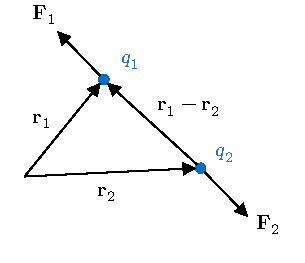
\includegraphics{coulomb_point_charges.pdf}
	\caption{Die Kraft auf zwei Punktladungen $q_1$ und $q_2$ an Orten $\vec r_1$ und $\vec r_2$ wird durch das Coulombsche Gesetz beschrieben und ist invers proportional zum Qudrat des Abstands $\left|\vec r_1-\vec r_2\right|$. }
	\label{fig:coulomb_point_charges}
\end{figure}

mit Dielektrizitätskonstante $\varepsilon _{0}=\SI{8,8541878128e-12}{\farad\per\m}$. Das Coulombsche Gesetz hat die gleiche Form wie das Newtonsche Gravitationsgesetz, aber hier kann die Kraft auch abstoßend wirken, weil die Ladung anders als die Masse negativ sein kann. Genauso wie beim Gravitationsgesetz ist die Kraft antiproportional zum Quadrat des Abstands der Ladungen.\footnote{Es ist möglich, dass die Proportionalität nicht exakt $\vec {F}\propto r^{-2}$ ist, aber es ist durch Experimente bestätigt worden, dass für einen Ansatz $F\propto r^{-2-\varepsilon }$ zumindest $\varepsilon <3\cdot 10^{-16}$ ist und für einen Ansatz $F\propto e^{-\frac{r}{\xi }}r^{-2}$ (siehe sogenanntes Yukawa-Potential) wenigstens $\xi >\SI{1e8}{\m}$. }

Mithilfe des Coulombschen Gesetzes können wir nach dem Superpositionsprinzip die Kraft auf eine Testladung $q_{0}$ am Ort $\vec {r}_{0}$ durch mehrere Ladungen $q_{i}$ bestimmen:
\begin{equation}
	\label{3.2}
	\vec {F}=\frac{q_{0}}{4\pi \varepsilon _{0}}\sum _{i}q_{i}\frac{\vec {r}_{0}-\vec {r}_{i}}{\left| \vec {r}_{0}-\vec {r}_{i}\right| ^{3}}
\end{equation}
Dieser Ansatz ist der Fernwirkungsstandpunkt (die Kraft wirkt über die Ferne hinweg). Seit Veröffentlichung der Relativitätstheorie ist aber bekannt, dass sich nichts schneller als mit Vakuumlichtgeschwindigkeit bewegen kann \textendash{} also auch keine Kraftwirkung.

Daher führt man den sogenannten Nahwirkungsstandpunkt ein, bei dem man man ein elektrisches Feld $\vec {E}$ betrachtet, das durch Ladungen $q_{i}$ erzeugt wird ($\vec {E}$ zeigt weg von positiven Ladungen und hin zu den negativen):
\begin{equation}
	\vec {E}\left(\vec {r}\right)=\frac{1}{4\pi \varepsilon _{0}}\sum _{i}q_{i}\frac{\vec {r}_{0}-\vec {r}_{i}}{\left| \vec {r}_{0}-\vec {r}_{i}\right| ^{3}},\quad \vec {E}\left(\vec {r}\right)=\frac{1}{4\pi \varepsilon _{0}}\int \rho \left(\vec {r}'\right)\frac{\vec {r}-\vec {r}'}{\left| \vec {r}-\vec {r}'\right| ^{3}}\diff ^{3}\vec {r}'
\end{equation}
Damit ergibt sich die folgende Kraft auf eine Testladung $q_{0}$:
\begin{equation}
	\vec {F}=q_{0}\vec {E}\left(\vec {r}_{0}\right)
\end{equation}


\section{Feldgleichungen der Elektrostatik}

\subsection{Grundlagen}

Wir definieren zunächst das elektrostatische Potential:
\begin{equation}
	\label{3.3}
	\boxed{\vec {E}=-\nabla \phi ,\quad \phi \left(\vec {r}\right)=\frac{1}{4\pi \varepsilon _{0}}\int \frac{\rho \left(\vec {r}'\right)}{\left| \vec {r}-\vec {r}'\right| }\diff ^{3}\vec {r}'}
\end{equation}
Weil $\vec {E}$ ein Potentialfeld ist, ist $\rot \vec {E}=0$. Das elektrostatische Feld ist also wirbelfrei.

Zum Beispiel ist das Potential einer Punktladung $\rho \left(\vec {r}\right)=q\delta \left(\vec {r}-\vec {r}_{0}\right)$ nach obiger Formel\footnote{Hinweis: Es gilt
	\begin{equation*}
		\nabla \frac{1}{\left| \vec {r}-\vec {r}\mathrm{'}\right| }=-\frac{1}{\left| \vec {r}-\vec {r}\mathrm{'}\right| ^{2}}\nabla \left| \vec {r}-\vec {r}\mathrm{'}\right| \overset{\nabla r=\frac{\vec {r}}{r}=\hat{\vec {r}}}{=}-\frac{\vec {r}-\vec {r}\mathrm{'}}{\left| \vec {r}-\vec {r}\mathrm{'}\right| ^{3}}
	\end{equation*}
}:
\begin{equation*}
	\phi \left(\vec {r}\right)=\frac{1}{4\pi \varepsilon _{0}}\frac{q}{\left| \vec {r}-\vec {r}_{0}\right| }
\end{equation*}
Die Quellen des elektrischen Feldes werden durch die Divergenz von $\vec E$ beschrieben,
\begin{equation*}
	\divg \vec {E}=-\nabla ^{2}\phi =-\frac{1}{4\pi \varepsilon _{0}}\int \rho \left(\vec {r}\mathrm{'}\right)\underset{\overset{!}{=}-4\pi \delta \left(\vec {r}-\vec {r}\mathrm{'}\right)}{\underbrace{\nabla ^{2}\frac{1}{\left| \vec {r}-\vec {r}\mathrm{'}\right| }}}\diff ^{3}r\mathrm{'}=\frac{1}{\varepsilon _{0}}\rho \left(\vec {r}\right).
\end{equation*}


\subsection{Feldgleichungen der Elektrostatik}

Die soeben gefundenen Zusammenhänge werden als Feldgleichungen der Elektrostatik bezeichnet:
\begin{align}
	\label{3.4}
	\Aboxed{\divg \vec {E} & =\frac{1}{\varepsilon _{0}}\rho \left(\vec {r}\right)} \\
	\label{3.5}
	\Aboxed{\rot \vec {E}  & =0}
\end{align}
Die erste Gleichung wird als Gaußsches Gesetz bezeichnet und beschreibt die elektrische Ladung als Quelle des elektrischen Feldes. Die zweite beschreibt die Wirbelfreiheit des elektrostatischen Feldes.

Mit $\vec {D}=\varepsilon _{0}\vec {E}$ im Vakuum kann man das Gaußsche Gesetz auch umformulieren zu
\begin{equation}
	\label{3.6}
	\divg \vec {D}=\rho \left(\vec {r}\right).
\end{equation}
Zu beiden Feldgleichungen gibt es integrale Formulierungen:
\begin{equation*}
	\int _{V}\diff ^{3}\vec r\divg \vec {E}=\int _{\partial V}\vec {E}\cdot \diff \vec {f}=\frac{1}{\varepsilon _{0}}\int \diff ^{3}\vec r\rho \left(\vec {r}\right)\implication \boxed{\int _{\partial V}\vec {E}\cdot \diff \vec f=\frac{1}{\varepsilon _{0}}Q}
\end{equation*}
\begin{formal}
	Der Fluss aus einem Volumen $V$ heraus ist proportional zu der Gesamtladung. Die elektrische Ladungsdichte ist die Quelle des elektrischen Feldes.
\end{formal}
Betrachte als Beispiel eine Punktladung, die das Feld $\vec {E}=\frac{1}{4\pi \varepsilon _{0}}q\frac{\vec {r}-\vec {r}_{0}}{\left| \vec {r}-\vec {r}_{0}\right| ^{3}}=\frac{1}{4\pi \varepsilon _{0}}q\frac{\hat{\vec {R}}}{R^{2}}$ erzeugt:
\begin{equation*}
	\int _{\partial V_{K}}\vec {E}\cdot \diff \vec {f}=\frac{q}{4\pi \varepsilon _{0}}\int _{\partial V_{K}}\frac{\hat{\vec {R}}}{R^{2}}\cdot \hat{\vec {R}}R^{2}\diff \Omega  =\frac{q}{4\pi \varepsilon _{0}}\int _{\partial V_{K}}\diff \Omega  =\frac{q}{\varepsilon _{0}}
\end{equation*}
Für die andere Feldgleichung betrachten wir das Arbeitsintegral, also die von einer Punktladung $q$ verrichtete Arbeit gegen die elektrische Kraft $\vec F_{\mathrm{el}}=q\vec {E}$.
\begin{equation*}
	W=-q\int _{C}\vec {E}\cdot \diff \vec {r}=q\int _{C}\nabla \phi \cdot \diff \vec {r}=q\int _{C}\diff \phi =q\left[\phi \left(2\right)-\phi \left(1\right)\right]
\end{equation*}
Insbesondere gilt
\begin{equation}
	\label{3.7}
	\oint \vec {E}\cdot \diff \vec {r}=0
\end{equation}

\begin{formal}
	Die Feldlinien des elektrostatischen Feldes sind nicht geschlossen, es gibt keine Zirkulation in der Elektrostatik, $\rot \vec {E}=0$.
\end{formal}



\subsection{Potentialgleichung}

Aus dem Gaußschen Gesetz können wir die folgende Poisson-Gleichung ableiten, die für $\rho =0$ zu einer Laplace-Gleichung wird:
\begin{equation}
	\label{3.8}
	\boxed{\nabla ^{2}\phi =-\frac{1}{\varepsilon _{0}}\rho }
\end{equation}
Zur Lösung einer linearen Differentialgleichung können wir die Methode der Greenschen Funktion verwenden. Dabei drücken wir die Lösung allgemein als Faltung der Ladungsdichte mit einer sogenannten Greenschen Funktion aus,
\begin{equation}
	\label{3.9}
	\phi \left(\vec {r}\right)=\int G\left(\vec {r}-\vec {r}'\right)\rho \left(\vec {r}'\right)\diff ^{3}\vec {r}'.
\end{equation}
Durch Vergleich mit der Bestimmungsgleichung des elektrischen Potentials können wir die Greensche Funktion für diese Differentialgleichung ablesen:
\begin{equation}
	\label{3.10}
	G\left(\vec {r}-\vec {r}'\right)=\frac{1}{4\pi \varepsilon _{0}}\frac{1}{\left| \vec {r}-\vec {r}'\right| }
\end{equation}
Insbesondere gilt für eine Punktladung $\rho \left(\vec {r}\right)=\delta \left(\vec {r}-\vec {r}_{0}\right)$, dass $\phi \left(\vec {r}\right)=G\left(\vec {r}-\vec {r}_{0}\right)$ und damit, dass
\begin{equation*}
	\nabla ^{2}\frac{1}{\left| \vec {r}-\vec {r}_{0}\right| }=-4\pi \delta \left(\vec {r}-\vec {r}_{0}\right).
\end{equation*}



\subsection{Feldlinien}

\begin{figure}[htb]
	\centering
	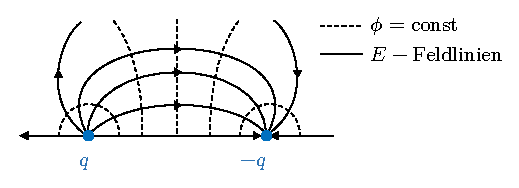
\includegraphics{dipole_field_potential.pdf}
	\caption{Äquipotentiallinien und elektrische Feldlinien von zwei ungleichnamigen Ladungen. }
	\label{fig:dipole_field_potential}
\end{figure}

Als Äquipotentiallinien bzw. -flächen werden die Linien/Flächen gleichen Potentials, $\phi =\text{const}$ bezeichnet. Die Feldlinien stehen senkrecht auf den Äquipotentialflächen, weil $\vec {E}\left(\vec {r}\right)=-\nabla \phi $. In \Abbref{fig:dipole_field_potential} sind die Äquipotentiallinien und die Feldlinien einer positiven und einer negativen Ladung dargestellt.

\subsection{Elektrostatische Energie}

Die potentielle Energie einer Ladung $q$ am Ort $\vec {r}$ im Feld $\vec {E}=-\nabla \phi $ ist definiert über einen Referenzpunkt $\phi _{1}=0$, der zum Beispiel im Unendlichen liegt (aber je nach Anwendung auch an anderen Punkten liegen kann):
\begin{equation}
	\label{3.11}
	U\left(\vec {r}\right)=q\phi \left(\vec {r}\right)
\end{equation}
Zum Beispiel ist die potentielle Energie von zwei Punktladungen
\begin{equation*}
	U=q_{1}\phi _{2}=\frac{1}{4\pi \varepsilon _{0}}\frac{q_{1}q_{2}}{\left| \vec {r}_{1}-\vec {r}_{2}\right| }.
\end{equation*}
Die elektrostatische Energie $U$ von $N$ Punktladungen im eigenen Feld kann dann in zwei Schritten bestimmt werden.
\begin{itemize}
	\item Bestimme die Energie von $q_{i}$ im Feld von $q_{j}$ ($j=1,\ldots ,i-1$):
	      \begin{equation*}
		      U_{i}\left(\vec {r}_{i}\right)=q_{i}\sum _{j=1}^{i-1}\phi _{j}=\frac{q_{i}}{4\pi \varepsilon _{0}}\sum _{j=1}^{i-1}\frac{q_{j}}{\left| \vec {r}_{i}-\vec {r}_{j}\right| }
	      \end{equation*}
	\item Bringe $N$ Ladungen sukzessive an ihren Ort:
	      \begin{equation*}
		      U=\sum _{i=2}^{N}U_{i}\left(\vec {r}_{i}\right)=\frac{1}{4\pi \varepsilon _{0}}\sum _{i=2}^{N}\sum _{j=1}^{i-1}\frac{q_{i}q_{j}}{\left| \vec {r}_{i}-\vec {r}_{j}\right| }=\frac{1}{8\pi \varepsilon _{0}}\sum _{i\neq j}^{N}\frac{q_{i}q_{j}}{\left| \vec {r}_{i}-\vec {r}_{j}\right| }
	      \end{equation*}

\end{itemize}
Für eine kontinuierliche Ladungsverteilung ergibt sich
\begin{equation*}
	U=\frac{1}{8\pi \varepsilon _{0}}\int \diff ^{3}\vec {r}\diff ^{3}\vec {r}'\frac{\rho \left(\vec {r}\right)\rho \left(\vec {r}'\right)}{\left| \vec {r}-\vec {r}'\right| }=\frac{1}{2}\int \diff ^{3}\vec {r}\rho \left(\vec {r}\right)\phi \left(\vec {r}\right)
\end{equation*}
Bemerkungen:
\begin{itemize}
	\item Den zusätzlichen Faktor von $\frac{1}{2}$ erhält man, weil $\phi \left(\vec {r}\right)$ von $\rho \left(\vec {r}\right)$ selbst erzeugt wird und die gegenseitige Wirkung von je zwei Ladungen die gleiche ist.

	\item Für beschränkte $\rho $ ist $\vec {r}\rightarrow \vec {r}'$ wohl definiert, da $\diff ^{3}r=r^{2}\diff r\diff \Omega  $.


\end{itemize}
Es ist auch möglich, die Energie durch das Feld $\vec {E}\left(\vec {r}\right)$ auszudrücken:
\begin{equation*}
	U=\frac{\varepsilon _{0}}{2}\int \diff ^{3}\vec {r}\phi \nabla ^{2}\phi \overset{\text{partielle Int}.}{=}\frac{\varepsilon _{0}}{2}\int \diff ^{3}\vec {r}\nabla \phi \cdot \nabla \phi =\frac{\varepsilon _{0}}{2}\int \diff ^{3}\vec {r}\left| \vec {E}\right| ^{2}
\end{equation*}
Damit lässt sich die Energiedichte in der Elektrostatik folglich schreiben als
\begin{equation*}
	u\left(\vec {r}\right)=\frac{\varepsilon _{0}}{2}\left| \vec {E}\left(\vec {r}\right)\right| ^{2}=\frac{1}{2}\vec {E}\cdot \vec {D}.
\end{equation*}



\subsection{Homogen geladene Kugel}

\begin{figure}[htb]
	\centering
	\tfigEfieldAndPotLinesAndChargeDensitityHomoChargedSphere
	\caption{Links: Äquipotentiallinien und elektrische Feldlinien einer homogen geladenen Kugel mit Radius $R$. Rechts: Die Ladungsdichte ist konstant $\rho_0$ innerhalb ($r<R$) und gleich 0 außerhalb der Kugel. }
	\label{fig:homogenously_charged_ball}
\end{figure}

Auf der homogen geladenen Kugel $V_{r}$ ist die Ladungsdichte $\rho \left(\vec {r}\right)$ innerhalb der Kugel konstant $\rho _{0}$ und außerhalb der Kugel gleich $0$ (siehe \Abbref{fig:homogenously_charged_ball}). Das Problem ist kugelsymmetrisch und hängt nur von der Radialrichtung ab.



\begin{figure}[htb]
	\centering
	\tfigEfieldAndPotentialHomoChargedSphere
	\caption{Links: Elektrisches Feld einer homogen geladenen Kugel. Das Feld steigt im Inneren linear an und fällt im Äußeren mit $r^{-2}$ ab. Rechts: Das Potential fällt im Äußeren genauso ab wie das Potential einer Punktladung. }
	\label{fig:homogenously_charged_ball_field_potential}
\end{figure}

Feld und Potential können zum Beispiel über das Gaußsche Gesetz berechnet werden:
\begin{align*}
	\int _{{V_{r}}}\diff ^{3}r'\frac{\rho \left(r\right)}{\varepsilon _{0}} & =\int _{{V_{r}}}\diff ^{3}r'\divg \vec {E}=\int _{\partial {V_{r}}}\vec {E}\cdot \diff \vec {f}\implication 4\pi r^{2}E\left(r\right)=\frac{1}{\varepsilon _{0}}\int _{0}^{r}\diff r'r'^{2}\rho \left(r'\right) \\
	\Rightarrow E\left(r\right)                                             & =\frac{Q}{4\pi \varepsilon _{0}}
	\begin{cases} \frac{r}{R^{3}}, & r<R     \\
              \frac{1}{r^{2}}, & r\geq R
	\end{cases} \quad\xrightarrow{\text{Integration}}\quad \phi \left(r\right)=\frac{Q}{4\pi \varepsilon _{0}}
	\begin{cases} \frac{3}{2R}-\frac{r^{2}}{2R^{3}}, & r<R     \\
              \frac{1}{r},                                              & r\geq R
	\end{cases}
\end{align*}
Beide Größen sind in \Abbref{fig:homogenously_charged_ball_field_potential} dargestellt. Bemerkenswert ist, dass für $r\geq R$ das elektrische Feld $\vec {E}\left(\vec {r}\right)=E\left(r\right)\cdot \vec {e}_{r}$ gerade dem Feld einer Punktladung $Q$ im Mittelpunkt der Kugel entspricht.

Es soll nun die Energiedichte $u\left(\vec {r}\right)$ für die homogen geladene Kugel berechnet werden:
\begin{align*}
	u\left(\vec {r}\right)=\frac{\varepsilon _{0}}{2}\left| \vec {E}\right| ^{2}=\frac{Q^{2}}{32\pi ^{2}\varepsilon _{0}}\begin{cases} \frac{r^{2}}{R^{6}}, & r<R     \\
              \frac{1}{r^{4}},     & r\geq R
	                                                                                                                     \end{cases}
\end{align*}
Daraus ergibt sich die elektrostatische Energie ("`Selbstenergie`` einer homogen geladenen Kugel)
\begin{equation*}
	U=4\pi \int _{0}^{\infty }\diff ru\left(r\right)r^{2}=\frac{1}{4\pi \varepsilon _{0}}\frac{3}{5}\frac{Q^{2}}{R}.
\end{equation*}
Diese Rechnung lässt über die Ruheenergie eines Elektrons eine Abschätzung für den Elektronenradius zu (sogenannter klassischer Elektronenradius):
\begin{equation*}
	U\overset{!}{=} m_{e}c^{2}\approx \SI{0.5}{\mega\eV}\implication R_{e}= \SI{1,7e-15}{\m}
\end{equation*}
Allerdings liegt die Compton-Wellenlänge $\lambda _{e}=\frac{h}{m_{e}c}=\SI{2e-12}{\m}$ schon weit über diesem Radius, sodass Quanteneffekte hier nicht vernachlässigbar sind.



\subsection{Extremalprinzip und Kapazitäten}

\begin{formal}
	In der Elektrostatik sind Leiter stets Äquipotentialflächen, d.h. $\phi =\text{const}$ und daher $\vec {E}=-\nabla \phi =\vec {0}$ entlang des Leiters. Sonst würde ein Strom fließen, weil sich die freien Elektronen im Leiter aufgrund des nicht-verschwindenden Feldes bewegen würden.
\end{formal}

\begin{figure}[htb]
	\centering
	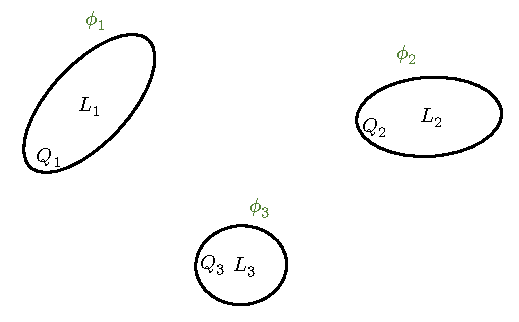
\includegraphics{three_conductors.pdf}
	\caption{Konfiguration von elektrischen Leitern $L_i$ mit Ladungen $Q_i$ und Potentialen $\phi_i$. }
	\label{fig:three_conductors}
\end{figure}

Betrachte den Fall von $n$ Leitern mit Volumina $L_{i}$, einer Ladung $Q_{i}$ und den Potentialen $\phi _{i}$, wie schematisch in \Abbref{fig:three_conductors} gezeigt.

Es soll untersucht werden, wie aus der Ladungsverteilung die Potentiale und das elektrische Feld bestimmt werden können.
\begin{formal}
	\textbf{Theorem von Thomson:}

	Die Ladungsdichten $\rho _{i}\left(\vec {r}\right)$ in Leitern $i$ stellen sich so ein, dass die Gesamtenergie minimal wird.
\end{formal}
Beweis:
\begin{equation*}
	U=\frac{1}{8\pi \varepsilon _{0}}\sum _{ij}\int _{L_{i}}\diff ^{3}\vec {r}_{i}\int _{L_{j}}\diff ^{3}\vec {r}_{j}\frac{\rho _{i}\left(\vec {r}_{i}\right)\rho _{j}\left(\vec {r}_{j}\right)}{\left| \vec {r}_{i}-\vec {r}_{j}\right| }
\end{equation*}
Minimierung unter der Nebenbedingung $\int _{{L_{i}}}\diff ^{3}\vec {r}\rho _{i}\left(\vec {r}\right)=Q_{i}$ führt auf
\begin{equation*}
	\frac{\partial }{\partial \rho _{k}\left(\vec {r}\right)}\left(U-\sum _{i}\phi _{i}\int _{L_{i}}\diff ^{3}\vec {r}_{i}\rho _{i}\left(\vec {r}\right)\right)=0
\end{equation*}
wobei in Voraussicht die Lagrange-Parameter als $\phi _{i}$ bezeichnet werden, weil sich mit
\begin{equation*}
	\partial _{{\rho _{k}}\left(\vec {r}\right)}\sum _{i}\int \rho _{i}\left(\vec {r}\right)f_{i}\left(\vec {r}\right)\diff ^{3}r=f_{k}\left(\vec {r}\right)
\end{equation*}
ergibt, dass
\begin{equation*}
	\phi _{k}=\frac{1}{4\pi \varepsilon _{0}}\sum _{j}\int _{L_{j}}\diff ^{3}\vec {r}_{j}\frac{\rho _{j}\left(\vec {r}_{j}\right)}{\left| \vec {r}_{k}-\vec {r}_{j}\right| },\quad \vec {r}_{k}\in L_{k}
\end{equation*}
was gerade der Bestimmungsgleichung für das Potential $\phi _{k}$ als Potential von $L_{k}$ entspricht. Da das Vorgehen der Minimierung der Gesamtenergie auf das richtige Potential führt, ist das Theorem bestätigt.


Die Potentiale $\phi _{i}$ lassen sich linear über die Ladungen $Q_{i}$ zerlegen,
\begin{equation*}
	\phi _{i}=\sum _{j}p_{ij}Q_{j},
\end{equation*}
weil einerseits gilt, dass $\nabla ^{2}\phi =-\rho /\varepsilon _{0}$ und andererseits $\phi $ linear in $\rho $ ist. Dieser Zusammenhang lässt sich invertieren,
\begin{equation*}
	Q_{i}=\sum _{j}C_{ij}\phi _{j},
\end{equation*}
wobei dann die Vorfaktoren $C_{ij}$ als Kapazitäten mit der Einheit $\left[C_{ij}\right]=\SI{1}{\coulomb\per\V}=\SI{1}{\farad}$ definiert werden. Aus dem Ausdruck für die elektrostatische Energie
\begin{equation*}
	U=\frac{1}{2}\sum _{i}\underset{Q_{i}=\sum _{j}C_{ij}\phi _{j}}{\underbrace{\int _{L_{i}}\diff ^{3}\vec {r}_{i}\rho _{i}\left(\vec {r}_{i}\right)\phi _{i}}}=\frac{1}{2}\sum _{ij}\phi _{i}C_{ij}\phi _{j}
\end{equation*}
folgt die Symmetrie $C_{ij}=C_{ji}$.

So gilt zum Beispiel für einen Plattenkondensator allgemein
\begin{equation*}
	C=\frac{Q}{V},\quad U=\frac{1}{2}CV^{2}=\frac{1}{2}QV
\end{equation*}
für einen Plattenkondensator mit parallelen Platten der Fläche $A$ und Abstand $d$
\begin{equation*}
	C=\varepsilon _{0}\varepsilon _{r}\frac{A}{d},
\end{equation*}
für einen Zylinderkondensator der Länge $L$ und mit Radien $r_{1}<r_{2}$
\begin{equation*}
	C=2\pi \varepsilon _{0}\varepsilon _{r}\frac{L}{\ln \frac{r_{2}}{r_{1}}}
\end{equation*}
und schließlich für einen Kugelkondensator mit Radien $r_{1}<r_{2}$
\begin{equation*}
	C=4\pi \varepsilon _{0}\varepsilon _{r}\left(\frac{1}{r_{1}}-\frac{1}{r_{2}}\right)^{-1}=4\pi \varepsilon _{0}\varepsilon _{r}\frac{r_{1}r_{2}}{d}.
\end{equation*}
\Abbref{fig:capacitors} bildet diese drei einfachen Kondensatorgeometrien ab.


\begin{figure}[htb]
	\centering
	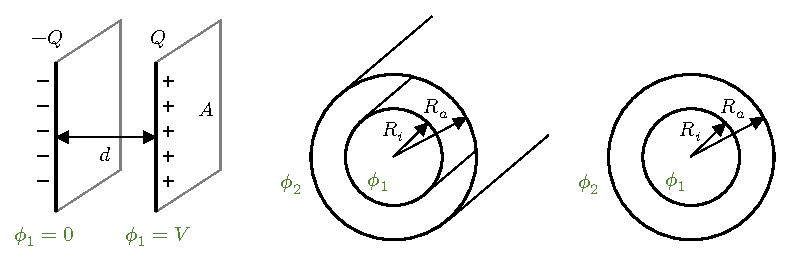
\includegraphics{capacitors.pdf}
	\caption{Schematische Darstellung eines Plattenkondensators mit parallelen, ebenen Platten (Links), eines Zylinderkondensators (Mitte) und eines Kugelkondensators (Rechts). Auf den Platten ist das Potential jeweils $\phi_1$ und $\phi_2$. }
	\label{fig:capacitors}
\end{figure}



\subsection{Maxwellscher Spannungstensor\label{sec:maxwellscher_spannungstensor}}

\section{Randbedingungen des elektrischen Feldes auf Grenzflächen\label{sec:randbedingungen_auf_grenzflaechen}}

 {\ldots}

\section{Randwertprobleme der Elektrostatik}

Meist sind bei der Lösung von elektrostatischen Problemen der Poisson-Gleichung
\begin{equation*}
	\nabla ^{2}\phi =-\frac{\rho }{\varepsilon _{0}}
\end{equation*}
in einem Volumen $V$ noch die Randbedingungen auf $\partial V$ zu berücksichtigen.

\subsection{Eindeutigkeit der Lösung}

Allgemein sind drei verschiedene Arten von Randbedingungen möglich.

\begin{enumerate}
	\item Dirichlet-Randbedingung: Das Potential ist auf dem Rand vorgegeben, $\left.\hspace{0pt}\phi \right| _{\partial V}$.

	\item Neumann-Bedingung: Die Normalenableitung der Lösung wird auf dem Rand vorgegeben, $\vec {n}\cdot \left.\hspace{0pt}\nabla \phi \right| _{\partial V}=\left.\frac{\partial \phi }{\partial n}\right| _{\partial V}$

	\item Cauchy-Bedingung: $a\left(1\right)+b\left(2\right)$ ist vorgegeben.
\end{enumerate}

Zum Beispiel kommt die Dirichlet-Randbedingung bei Oberflächen von Leitern vor, von denen wir ja bereits wissen, dass dort das Potential konstant gleich $0$ ist.
\begin{formal}
	Für Dirichlet- und Neumann-Randbedingungen ist die Lösung der Poisson-Gleichung eindeutig.
\end{formal}
Der Beweis ist einfach, denn seien $\phi _{1}$ und $\phi _{2}$ zwei unterschiedliche Lösungen, dann erfüllt $\phi _{d}=\phi _{1}-\phi _{2}$ die Gleichung $\nabla ^{2}\phi _{2}=0$ mit der Randbedingung
\begin{align*}
	\begin{cases} \left.\phi _{d}\right| _{\partial V}                             & =0 \\
              \left.\frac{\partial \phi _{d}}{\partial n}\right| _{\partial V} & =0
	\end{cases} ,
\end{align*}
da $\phi _{1,2}$ die gleichen Randbedingungen erfüllen. Mit der zweiten Greenschen Identität folgt
\begin{equation*}
	\int _{V}\left(\varphi \nabla ^{2}\psi +\nabla \varphi \cdot \nabla \psi \right)\diff V=\int _{\partial V}\varphi \nabla \psi \cdot \diff \vec {f}.
\end{equation*}
Setze nun $\varphi =\psi =\phi _{d}$:
\begin{equation*}
	\int _{V}\left(\nabla \phi _{d}\right)^{2}\diff V=0
\end{equation*}
Da nun aber der Integrand stets positiv ist, folgt $\nabla \phi _{d}=0$ und also ohne Beschränkung der Allgemeinheit $\phi _{d}=\text{const}=0$.


\subsection{Methode der Greenschen Funktion}

\subsection{Aussagen zur Potentialtheorie}

\subsection{Lösungen zur Laplace-Gleichung in Kugelkoordinaten}

Die Laplace-Gleichung ist eine zentrale Gleichung in der Physik. In der Elektrostatik gilt sie zum Beispiel im ladungsfreien Raum, aber sie spielt auch für viele andere Modelle eine große Rolle. In kartesischen Koordinaten nimmt die Gleichung die Form
\begin{equation*}
	\nabla ^{2}\phi =\left(\frac{\partial ^{2}}{\partial x^{2}}+\frac{\partial ^{2}}{\partial y^{2}}+\frac{\partial ^{2}}{\partial z^{2}}\right)\phi =0
\end{equation*}
an. Die Lösung lässt sich in Eigenfunktionen des Laplace-Operators zerlegen. Diese sind zum Beispiel für den kartesischen Fall ebene Wellen.

Für kugelsymmetrische Problem bietet es sich an in Kugelkoordinaten zu rechnen. In Kugelkoordinaten lässt sich der Laplace-Operator in Radial- und Winkelanteil zerlegen:
\begin{align*}
	\nabla ^{2}\phi & =\nabla _{r}^{2}\phi +\frac{1}{r^{2}}\nabla _{\varphi ,\vartheta }^{2}\phi \\&=\frac{1}{r^{2}}\frac{\partial }{\partial r}r^{2}\frac{\partial }{\partial r}\phi +\frac{1}{r^{2}\sin \vartheta }\frac{\partial }{\partial \vartheta }\sin \varphi \frac{\partial }{\partial \vartheta }\phi -\frac{1}{r^{2}\sin ^{2} \vartheta }\frac{\partial ^{2}}{\partial \varphi ^{2}}\phi
\end{align*}
Zur Lösung wird ein Produktansatz gemacht,
\begin{equation*}
	\phi \left(r,\varphi ,\vartheta \right)=R\left(r\right)Y\left(\varphi ,\vartheta \right).
\end{equation*}
Eingesetzt in die Laplace-Gleichung ergibt sich
\begin{equation*}
	Y\nabla _{r}^{2}R+\frac{R}{r^{2}}\nabla _{\varphi ,\vartheta }^{2}Y=0 \equivalence\frac{r^{2}}{R}\nabla _{r}^{2}R=-\frac{1}{Y}\nabla _{\varphi ,\vartheta }^{2}Y=\text{const}
\end{equation*}
und hieraus erhält man separat die radialen Eigenfunktionen
\begin{equation*}
	R\left(r\right)=\alpha r^{l}+\beta r^{-\left(l+1\right)}
\end{equation*}
und die bereits aus der Quantenmechanik bekannten Kugelflächenfunktionen $Y_{lm}\left(\varphi ,\vartheta \right)$ für den Winkelanteil nach der Eigenwertgleichung
\begin{equation*}
	\nabla _{\varphi ,\vartheta }^{2}Y_{lm}=-l\left(l+1\right)Y_{lm}.
\end{equation*}
Die Gesamtlösung setzt sich dann zusammen aus dem Radial- und Winkelanteil:
\begin{equation*}
	\phi \left(r,\varphi ,\vartheta \right)=\sum _{l=0}^{\infty }\sum _{m=-l}^{l}\underset{\text{Radialanteil}}{\underbrace{\left(\alpha _{lm}r^{l}+\beta _{lm}r^{-\left(l+1\right)}\right)}}\underset{\text{Winkelanteil}}{\underbrace{Y_{lm}\left(\varphi ,\vartheta \right)}}
\end{equation*}
Für zylindersymmetrische Probleme ist die $\varphi $-Abhängigkeit aufgehoben und es brauchen nur Funktionen mit $m=0$ betrachtet zu werden.

Für die Kugelflächenfunktionen von zwei Vektoren $\vec {r}_{1}=\left(r_{1},\varphi _{1},\vartheta _{1}\right)$ und $\vec {r}_{2}=\left(r_{2},\varphi _{2},\vartheta _{2}\right)$ gilt das folgende Additionstheorem:
\begin{equation*}
	\sum _{m=-l}^{l}Y_{lm}\left(\varphi _{1},\vartheta _{1}\right)Y_{lm}^{*}\left(\varphi _{2},\vartheta _{2}\right)=\frac{2l+1}{4\pi }P_{l}\left(\cos \angle \left(\vec {r}_{1},\vec {r}_{2}\right)\right)
\end{equation*}
Die Greensche Funktion kann mit diesem Additionstheorem nach den Kugelflächenfunktionen entwickelt werden
\begin{equation*}
	\frac{1}{\left| \vec {r}-\vec {r}'\right| }=\frac{1}{\sqrt{r^{2}+r'^{2}-2rr'\cos \vartheta }}=\sum _{l}\frac{r_{<}^{l}}{r_{>}^{l+1}}P_{l}\left(\cos \vartheta \right),\quad
	r_{>}=\max \left(r,r'\right) ,\quad
	r_{<}=\min \left(r,r'\right)
\end{equation*}


\begin{figure}[htb]
	\centering
	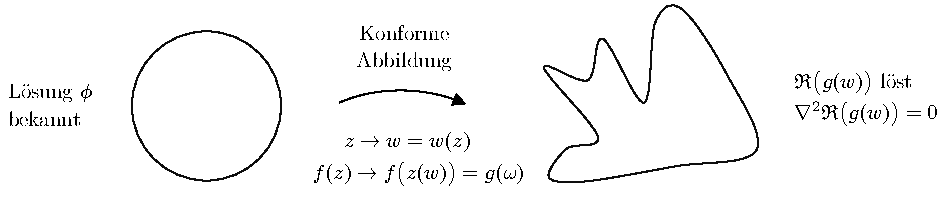
\includegraphics{complex_problems_conformal_map.pdf}
	\caption{Für Probleme mit komplexen Geometrien kann mithilfe einer konformen Abbildung $z$ die Lösung aus der Lösung für den kugelsymmetrischen Fall abgeleitet werden. }
	\label{fig:complex_problems_conformal_map}
\end{figure}

Obwohl die Wahl der Kugelkoordinaten nur für wenige Probleme sinnvoll ist, kann die Lösung für das kugelförmige Problem durch konforme Abbildungen auf komplexere Geometrien angewandt werden (\Abbref{fig:complex_problems_conformal_map}).

\section{Multipolentwicklung}

Bei der Multipolentwicklung klassifiziert man bestimmte Ladungsverteilungen nach sogenannten Momenten (Dipolmoment, Quadrupolmoment, {\ldots}). Zum Beispiel beschreibt das Dipolmoment zwei räumlich voneinander getrennte Ladungen unterschiedlichen Vorzeichens. Auch ein nach außen insgesamt elektrisch neutraler Körper kann ein Dipolmoment aufweisen, nämlich wenn die Schwerpunkte von der positiven und negativen Ladung nicht zusammenfallen. Ein prominentes mikroskopisches Beispiel ist das Wassermolekül (\Abbref{fig:water_molecule}), bei dem das Sauerstoffatom eine bedeutend größere Elektronegativität besitzt als die Wasserstoffatome und dadurch eine Ladungsverschiebung der gebundenen Elektronen zum Sauerstoffatom hin bewirkt. Dadurch besitzt dieses lokal eine Ladung von $\SI{-0.8}{\eV}$, während die Wasserstoffatome eine Ladung von je $\SI{+0.4}{\eV}$ tragen.

Das Dipolmoment $\vec {p}$ ist ein Vektor und per Definition von der negativen Ladung zur positiven gerichtet. Die Einheit des Dipolmoments ist $\SI{1}{Debye}=\SI{3,34e-30}{\coulomb\m}$.



\begin{figure}[htb]
	\centering
	\tfigWatermolecule
	\caption{Das Wassermolekül ist ein Dipol, bei dem das Sauerstoffatom eine negative Partialladung trägt, während die Wasserstoffatome aufgrund ihrer geringeren Elektronegativität entsprechend positiv geladen sind. }
	\label{fig:water_molecule}
\end{figure}

Für die Multipolentwicklung wird das Potential
\begin{equation*}
	\phi \left(\vec {r}\right)=\frac{1}{4\pi \varepsilon _{0}}\int \diff ^{3}\vec {r}'\frac{\rho \left(\vec {r}\right)}{\left| \vec {r}-\vec {r}'\right| }
\end{equation*}
nach den sogenannten Momenten der Ladungsverteilung entwickelt. Führe dazu zunächst eine Taylorentwicklung für den Ausdruck $1/\left| \vec {r}-\vec {r}'\right| $ um $\vec {r}$ durch ($\left| \vec {r}\right| =r$, Einsteinsche Summenkonvention):
\begin{equation*}
	\frac{1}{\left| \vec {r}-\vec {r}'\right| }=\frac{1}{r}-x_{i}'\partial _{i}\frac{1}{r}+\frac{1}{2}x_{i}'x_{j}'\partial _{i}\partial _{j}\frac{1}{r}+\ldots +\frac{\left(-1\right)^{n}}{n!}x_{i_{1}}'\ldots x_{i_{n}}'\partial _{{i_{1}}}\ldots \partial _{{i_{n}}}\frac{1}{r}
\end{equation*}
Damit lässt sich das Potential nähern als
\begin{align*}
	\phi \left(\vec {r}\right) & \approx \frac{1}{4\pi \varepsilon _{0}}\left(\int \diff ^{3}\vec {r}'\frac{\rho \left(\vec {r}\right)}{r}-\int \diff ^{3}\vec {r}'\rho \left(\vec {r}\right)x_{i}'\partial _{i}\frac{1}{r}+\frac{1}{2}\int \diff ^{3}\vec {r}'\rho \left(\vec {r}\right)x_{i}'x_{j}'\partial _{i}\partial _{j}\frac{1}{r}+\ldots \right. \\ &\quad\quad\left. +\frac{\left(-1\right)^{n}}{n!}\int \diff ^{3}\vec {r}'\rho \left(\vec {r}\right)x_{i_{1}}'\ldots  x_{i_{n}}'\partial _{{i_{1}}}\ldots \partial _{{i_{n}}}\frac{1}{r}\right)\\&=\frac{1}{4\pi \varepsilon _{0}}\left(\frac{1}{r}\underset{q}{\underbrace{\int \diff ^{3}\vec {r}'\rho \left(\vec {r}\right)}}-\partial _{i}\frac{1}{r}\underset{p_{i}}{\underbrace{\int \diff ^{3}\vec {r}'\rho \left(\vec {r}\right)x_{i}'}}+\frac{1}{6}\partial _{i}\partial _{j}\frac{1}{r}\underset{Q_{ij}}{\underbrace{\int \diff ^{3}\vec {r}'\rho \left(\vec {r}\right)\left(3x_{i}'x_{j}'-r^{'2}\delta _{ij}\right)}}+\ldots \right. \\ &\quad\quad\left.  +\,\partial _{{i_{1}}}\ldots \partial _{{i_{n}}}\frac{1}{r}\underset{M_{{i_{1}}\ldots {i_{n}}}}{\underbrace{\frac{\left(-1\right)^{n}}{n!}\int \diff ^{3}\vec {r}'\rho \left(\vec {r}\right)x_{i_{1}}'\ldots x_{i_{n}}'}}\right)\\&=\frac{1}{4\pi \varepsilon _{0}}\left(\frac{q}{r}-p_{i}\partial _{i}\frac{1}{r}+\frac{1}{6}Q_{ij}\partial _{i}\partial _{j}\frac{1}{r}+\ldots +M_{{i_{1}}\ldots {i_{n}}}\partial _{{i_{1}}}\ldots \partial _{{i_{n}}}\frac{1}{r}\right).
\end{align*}
Dabei identifizieren wir das Dipolmoment als Tensor erster Stufe
\begin{equation*}
	p_{i}=\int \diff ^{3}\vec {r}'\rho \left(\vec {r}\right)x_{i}',
\end{equation*}
das Quadrupolmoment als Tensor zweiter Stufe
\begin{equation*}
	Q_{ij}=\int \diff ^{3}\vec {r}'\left(3x_{i}'x_{j}'-r^{'2}\delta _{ij}\right)\rho \left(\vec {r}\right),
\end{equation*}
bei dem standardmäßig noch der Term $-r^{'2}\delta _{ij}$ hinzugefügt wird, welcher aber nicht zu $\phi(\vec r) $ beiträgt, weil
\begin{equation*}
	\delta _{ij}\partial _{i}\partial _{j}\frac{1}{r}=\sum _{i}\partial _{i}^{2}\frac{1}{r}=\nabla ^{2}\frac{1}{r}=0
\end{equation*}
und schließlich das $n$-te Multipolmoment
\begin{equation*}
	M_{{i_{1}}\ldots {i_{n}}}\propto \int \diff ^{3}\vec {r}'\rho \left(\vec {r}\right)x_{i_{1}}'\ldots x_{i_{n}}'.
\end{equation*}
Mit den Identitäten
\begin{equation*}
	\partial _{i}\frac{1}{r}=-\frac{1}{r^{2}}\partial _{i}r=-\frac{x_{i}}{r^{3}},\quad \partial _{i}\partial _{j}\frac{1}{r}=\frac{3x_{i}x_{j}}{r^{5}}-\frac{\delta _{ij}}{r^{3}},
\end{equation*}
(wobei der Term $\delta_{ij}/r^3$ irrelevant ist wegen $\delta _{ij}Q_{ij}=Q_{ii}=0$) erhält man dann für das Potential
\begin{equation*}
	\phi \left(\vec {r}\right)=\frac{1}{4\pi \varepsilon _{0}}\left(\frac{q}{r}+\frac{\vec {p}\cdot \vec {r}}{r^{3}}+\frac{1}{2}Q_{ij}\frac{x_{i}x_{j}}{r^{5}}+\ldots \right).
\end{equation*}



\subsection{Diskussion der Multipolmomente}

\begin{enumerate}
	\item Monopol (Potential/Feld einer Punktladung $\rho _{m}=q\delta \left(\vec {r}\right)$)
	      \begin{equation*}
		      \phi _{\mathrm{m}}\left(\vec {r}\right)=\frac{1}{4\pi \varepsilon _{0}}\frac{q}{r}\rightarrow \vec {E}(\vec r)=\frac{q}{4\pi \varepsilon _{0}}\frac{\vec {r}}{r^{3}}
	      \end{equation*}
	\item Dipol:
	      \begin{align*}
		      \phi _{\diff } & =-\frac{1}{4\pi \varepsilon _{0}}\vec {p}\cdot \nabla \frac{1}{r}=\frac{1}{4\pi \varepsilon _{0}}\frac{\vec {p}\cdot \vec {r}}{r^{3}}\propto \frac{1}{r^{2}}                                        \\
		      E_{i}          & =\frac{1}{4\pi \varepsilon _{0}}p_{j}\nabla _{i}\nabla _{j}\frac{1}{r}=\frac{1}{4\pi \varepsilon _{0}}\frac{p_{j}}{r^{3}}\left(\frac{3x_{i}x_{j}}{r^{2}}-\delta _{ij}\right)\propto \frac{1}{r^{3}}
	      \end{align*}
	      Wir sehen, dass das Feld eines Dipols mit $r^{-3}$ abnimmt, während dasjenige eines Monopols nur mit $r^{-2}$ abfällt. Die Felder der einzelnen Ladungen heben sich im Fernfeld zum Teil auf.

	      Die Ladungsdichte eines elementaren Dipols ist
	      \begin{equation*}
		      \rho _{\diff }\left(\vec {r}\right)=q\left(\delta \left(\vec {r}-\frac{\vec {d}}{2}\right)-\delta \left(\vec {r}+\frac{\vec {d}}{2}\right)\right),
	      \end{equation*}
	      woraus sich ein Dipolmoment von
	      \begin{equation*}
		      \vec {p}=q\vec {d}\parallel \vec {d}
	      \end{equation*}
	      ergibt.

	      Man kann auch einen sogenannten Punktdipol betrachten \textendash{} ein idealisiertes Objekt, bei dem der Abstand $\vec {d}$ gegen $0$ geht:
	      \begin{equation*}
		      \vec {p}=\lim _{\substack{
				      d\rightarrow 0 \\
				      qd<\infty}} q\vec {d},\quad \rho _{\diff }\left(\vec {r}\right)=-\vec {p}\cdot \nabla \delta \left(\vec {r}\right), \quad\phi _{\diff }=-\frac{1}{4\pi \varepsilon _{0}}\vec {p}\cdot \nabla \frac{1}{r}
	      \end{equation*}
	\item Quadrupol:
	      \begin{align*}
		      \phi _{\mathrm{Q}} & =\frac{1}{4\pi \varepsilon _{0}}\frac{1}{6}Q_{kl}\nabla _{k}\nabla _{l}\frac{1}{r}=\frac{1}{4\pi \varepsilon _{0}}\frac{1}{2}Q_{kl}\frac{x_{k}x_{l}}{r^{5}}\propto \frac{1}{r^{3}}                                                                   \\
		      E_{i}              & =-\frac{1}{4\pi \varepsilon _{0}}\frac{1}{6}Q_{kl}\nabla _{i}\nabla _{k}\nabla _{l}\frac{1}{r}=\frac{1}{4\pi \varepsilon _{0}}\frac{Q_{kl}}{2}\frac{5x_{i}x_{k}x_{l}-r^{2}\left(\delta _{kl}x_{i}+\delta _{il}x_{k}+\delta _{ik}x_{l}\right)}{r^{7}}
	      \end{align*}


	      \begin{figure}[htb]
		      \centering
		      \tfigElementalQuadrupoles
		      \caption{Elementare Quadrupole können in zwei verschiedenen Konfigurationen auftreten. }
		      \label{fig:elemental_quadrupoles}
	      \end{figure}

	      Es gibt zwei elementare Quadrupole (mit $\vec {p}=0$), die in \Abbref{fig:elemental_quadrupoles} zu sehen sind.

	      Wird der Bezugspunkt/Aufpunkt verschoben, so ändern sich im Allgemeinen die Multipolmomente, aber das erste Moment, das bei der Multipolentwicklung einer Ladungsverteilung ungleich $0$ ist, bleibt unverändert.


	      \begin{formal}
		      Das niedrigste, nicht-verschwindende Multipolmoment in der Entwicklung ist unabhängig vom Bezugspunkt.
	      \end{formal}
	      Man kann auch sphärische Multipolmomente mithilfe von Kugelflächenfunktionen ausdrücken.
\end{enumerate}


\subsection{Energie von Multipolen im äußeren Feld}

Die Energie von Multipolen in einem externen Potential $\phi _{e}\left(\vec {r}\right)$ kann aus der bereits bekannten Formel für die Energie einer beliebigen Ladungsverteilung $\rho \left(\vec {r}\right)$ abgeleitet werden,
\begin{equation*}
	U=\int _{V}\diff ^{3}\vec {r}\rho \left(\vec {r}\right)\phi _{e}\left(\vec {r}\right).
\end{equation*}
Wir nehmen an, dass die Änderung von $\phi _{e}$ in $V$ nur klein ist und erhalten durch eine Taylor-Entwicklung
\begin{align*}
	U & =\int \diff ^{3}\vec {r}\rho \left(\vec {r}\right)\left[\phi _{e}\left(0\right)+\vec {r}\nabla \phi _{e}\left(0\right)+\frac{1}{2}x_{i}x_{j}\nabla _{i}\nabla _{j}\phi _{e}\left(0\right)+\ldots \right] \\&=q\phi \left(0\right)-\vec {p}\cdot E_{e}\left(0\right)-\frac{1}{6}Q_{ij}\nabla _{j}E_{e}^{\left(i\right)}\left(0\right)+\ldots
\end{align*}
Die Energie der Multipole ist also durch die $n$-fache Ableitung des Potentials $\nabla ^{n}\phi $ bestimmt. Diese Rechnung erlaubt wegen der Taylor-Entwicklung eine beliebige Wahl des Bezugspunkts.

\begin{figure}[htb]
	\centering
	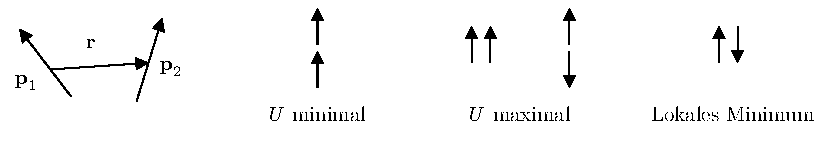
\includegraphics{dipoles.pdf}
	\caption{Links: Schematische Darstellung zweier Dipole $\vec p_1$, $\vec p_2$ mit Abstand $\vec r$. Weitere Abbildungen: Spezielle Anordnungen zweier Dipole, für die die Energie extremal wird. }
	\label{fig:dipoles}
\end{figure}

Als typisches Beispiel soll die Wechselwirkung zweier Dipole betrachtet werden. Die potentielle Energie kann berechnet werden, indem der Dipol $\vec {p}_{2}$ wie oben beschrieben in das Feld des Dipols $\vec {p}_{1}$ gesetzt wird (oder umgekehrt):
\begin{equation*}
	U_{\mathrm{DD}}=-\vec {p}_{2}\cdot \vec {E}_{1}\left(\vec {r}\right)=-\frac{1}{4\pi \varepsilon _{0}}\frac{1}{r^{3}}\left(\frac{3\left(\vec {r}\cdot \vec {p}_{1}\right)\left(\vec {r}\cdot \vec {p}_{2}\right)}{r^{2}}-\vec {p}_{1}\cdot \vec {p}_{2}\right)
\end{equation*}
Diese wird minimal für $\vec {p}_{1}\parallel \vec {p}_{2}\parallel \vec {r}$ und maximal für $\vec {p}_{1}\parallel \vec {p}_{2}\perp \vec {r}$. Diese Konfigurationen sind in \Abbref{fig:dipoles} zusammengestellt. Für antiparallele $\vec {p}_{1}$ und $\vec {p}_{2}$ und $\vec {p}_{1},\vec {p}_{2}\perp \vec {r}$ wird außerdem ein lokales Minimum erreicht. Aus diesem Grund bilden Dipolmoleküle auch häufig Molekülketten.

Zuletzt sollen noch Drehmomente auf Multipole diskutiert werden.
\begin{align*}
	\vec {M}           & =\int \diff ^{3}\vec {r}\vec {r}\times \underset{\text{Kraftdichte}}{\underbrace{\rho \left(\vec {r}\right)\vec {E}_{e}\left(\vec {r}\right)}}\implication M_{i}=\int \diff ^{3}\vec {r}\varepsilon _{ijk}x_{j}\rho \left(\vec {r}\right)\underset{\approx E_{e}^{\left(k\right)}\left(0\right)+x_{l}\nabla _{l}E_{e}^{\left(k\right)}\left(0\right)}{\underbrace{E_{e}^{\left(k\right)}\left(\vec {r}\right)}} \\
	\implication M_{i} & =\left(\vec {p}\times \vec {E}_{e}\right)_{i}+\frac{1}{3}\varepsilon _{ijk}Q_{jl}\nabla _{l}E_{e}^{\left(k\right)}
\end{align*}
Insbesondere dreht das Drehmoment $\vec {M}$ einen Dipol parallel zu $\vec {E}$, da $\vec {M}=0$ für $\vec {p}\parallel \vec {E}_{e}$ und
\begin{equation*}
	U=-\vec {p}\cdot \vec {E}_{e}=-pE_{e}\cos \vartheta \implication M=-\frac{\partial U}{\partial \vartheta }=-pE_{e}\sin \vartheta =-\left| \vec {p}\times \vec {E}_{e}\right| .
\end{equation*}